\documentclass[utf8,english]{gradu3}
% If you are writing a Bachelor's Thesis, use the following instead:
%\documentclass[utf8,bachelor,english]{gradu3}

\usepackage{booktabs} % good for beautiful tables
\usepackage{pdfpages}
\usepackage{todonotes}
\usepackage{url}
\usepackage{algorithm}
\usepackage{algpseudocode}
\usepackage{amssymb}
%some hacking because both the template and the amsmath package define \proof
\let\proof\relax 
\let\endproof\relax
\usepackage{amsmath}
\usepackage{amsthm}
\usepackage{graphicx}
\usepackage{paralist}
\usepackage{mdwlist}
\usepackage{threeparttable}
\usepackage{footmisc}
\usepackage{soul}
\usepackage{cleveref}
\usepackage{varwidth}
\usepackage{enumitem}
\usepackage[bookmarksopen,bookmarksnumbered,linktocpage]{hyperref}



% NOTE: This must be the last \usepackage in the whole document!


\DeclareGraphicsExtensions{.png,.pdf,.jpg}

\addbibresource{malliopas.bib} % The file name of your bibliography database
\bibliography{malliopas} {}

\begin{document}

\title{Clustering Analysis and Approximate Hierarchy Clustering Algorithm}
\translatedtitle{\LaTeX-tutkielmapohjan {gradu3} käyttö}
\studyline{All study lines}
\avainsanat{%
  \LaTeX,
  {gradu3},
  pro gradu -tutkielmat,
  kandidaatintutkielmat,
  käyttöohje}
\keywords{\LaTeX, {gradu3}, Master's Theses, Bachelor's Theses, user's guide}
\tiivistelma{%
  Empty TODO
}
\abstract{%
  Clustering Analysis and Approximate Hierarchy Clustering Algorithm.
}

\author{Mou Hao}
\contactinformation{Ag~C416.1, 
	\texttt{mouhao1990@outlook.com}}
% use a separate \author command for each author, if there is more than one
\supervisor{Unsupervised work}
% use a separate \supervisor command for each supervisor, if there
% is more than one

 % you don't need this line in a thesis
% \type{Template and manual for a thesis document class}

\maketitle

\preface
This is where you can write a preface for your thesis.  Most theses
don't have prefaces, but if you write one, keep it short (at least one
page).

The preface should discuss more the thesis process than the content of
the thesis.  For example, if there is something out of the ordinary in
your choice of a thesis topic or if something out of the ordinary
happened during its prepararion, the preface is where you could write
about it.  It is also customary in a preface to thank by name those
persons who helped you with your thesis -- at least your supervisor,
your spouse and your children, if any.  (Your family likely will have
helped you by encouraging and supporting you.)

The preface is typically in the first person (``I'').  It is also common
to sign it.

Jyväskylä, \today

\bigskip

The Author

\begin{thetermlist}
\item[\TeX] A batch-oriented typesetting system written by 
Donald Knuth in 1977--1989 \parencite[see][]{knuth86:_texbook}. 
\item[\LaTeX] A system, built on top of \TeX\
  \parencite{knuth86:_texbook}, for typesetting structured
  documents \parencite[see][]{lamport94:_latex}.  Its current version
  is \LaTeXe.
\end{thetermlist}

\newtheorem{definition}{Definition}
\crefname{definition}{definition}{definitions}
\Crefname{definition}{Definition}{Definitions}

\mainmatter

\chapter{Introduction}

% Introduction (describe the structure of the thesis and point out the contributions)

Data analysis has become the fundamental skill for modern science research across different subjects. Clustering is one of the most important component of data analysis. Researchers has invented many tools in the area of clustering analysis, while each method may focus on different area to solve all the diverse problems. 

The following of this thesis consists of a discussion about general clustering concept, the traditional genre of different clustering algorithms, a detailed comparison of approximate algorithms about hierarchical clustering algorithms and in the end, a paper in this topic  published in the SIGMOD(2015) attached.

The main contributions of this thesis are a thorough survey of clustering data mining techniques and introduces a state of art algorithm about hierarchical clustering algorithm.


\chapter{Clustering}

% Clustering (includes normal and hierarchical clustering)

Clustering, as the name suggests, is a method to divide similar objects into different groups. Each group, or says cluster, is made up by similar objects, and objects in different groups should be dissimilar. In machine learning point of view, clustering algorithms is unsupervised learning, which is used to find hidden patterns in data with unlabeled data. Unlike classification problems take use of the third part judgement about the data (labeled data), clustering analysis groups objects based only on the pattern and relationships of the raw data. 

As Dongkuan et al. ~\cite{xu2015comprehensive} pointed out, the standard process of clustering is usually divided into the following steps, and this thesis mainly focus on the algorithm itself, feature engineering and practical usage is not covered in detail.

\begin{itemize}
	\item Feature extraction, a set of parameter, or features generated from the original data to represent the objects.
	\item Selection of the proper clustering algorithm.
	\item Result evaluation, to evaluate the clustering result and make judgement about the algorithm and features.
	\item Practice use and result explanation.
\end{itemize}

The clustering methods are mainly divided into two categories viz., partition based clustering and hierarchical clustering, based on the way they produce the results. Partitioning based algorithms produce clusters directly, which means they try to find clusters by iteration to relocate objects into subsets. On the other hand, hierarchical clustering algorithms build clusters gradually, and hierarchical clustering is subdivided into agglomerative and divisive.

As shown above, clustering algorithm is about make the similar objects into one group, the definition of similar between objects is vital when discussion about clustering algorithm. This chapter will first illustrate the idea of similarity measure, and followed by a discussion about different genres of clustering algorithms in a row.

\section{Similarity Measure}

Similarity measure, which is the essential part of any clustering algorithm, a brief but concrete discussion about similarity measure is conducted in this section.

Similarity measure or distance metrics is the measure of relationship of different objects. The Choosing of distance metrics may greatly affect the clustering result. A list of popular similarity definitions will be shown in the following part.

\begin{definition}[Jaccard Distance]
	\label{def:jaccard_distance}
	Given two objects, $A$ and $B$, both objects have the same categories of features, the distance $D$ between $A$ and $B$ is defined as:
	\[
	D\left(A,B\right) = 1 - 
	\frac{
		\lvert A \cap B \lvert
	}{
		\lvert A \cup B \lvert
	}
\]
\end{definition}

\begin{definition}[Euclidean Distance]
	\label{def:euclidean_distance}
	Given two objects, $A$ and $B$, both objects have the same categories of features $K$, the distance $D$ between $A$ and $B$ is defined as:
	\[
	D\left(A,B\right) =
	\sum\limits_{i=1}^{\lvert  K\rvert } \left( 
		A_i - B_i
		\right)^2
\]
\end{definition}

\begin{definition}[Cosine Distance]
	\label{def:cosine_distance}
	Given two vector objects, $ \overrightarrow{A}$ and $\overrightarrow{B}$, both objects have the same categories of features $K$, the distance $D$ between $A$ and $B$ is defined as:
	\[
	1- \frac{ \overrightarrow{A}^T \overrightarrow{B} }{\left \| A \right \| \left \| B \right \|}
	\]
\end{definition}

Besides the distance metrics discussed above, a lot more possible options are also available, such as, Hamming Distance, Pearson Correlation Distance, Minkowski Distance et.al. 

While there are no golden standard for choosing distance metrics, practical usage of distance measure is often conducted via experiment.

A critical property of distance measure is triangle inequality, which means, for three different objects with three distance for each pair, the sum of any two distance must be greater than or equal to the remaining one.

The three distance measure mentioned above, the euclidean distance \ref{def:euclidean_distance} and jaccard distance \ref*{def:jaccard_distance} is naturally obey the triangle inequality feature, while the cosine distance \ref*{def:cosine_distance} violate it, and should be converted into angular distance to support this feature.


\section{Partial Clustering}

Partitioning Based Clustering can be treated as divide data into several subsets, which consists of a iteration process based on some greedy heuristic strategy. This method can further divided into distance based and density based.

For distance based clustering, the algorithms relocate object into cluster based on distance measure. The most famous algorithm is $K-means$. $K-mneas$ algorithm, as the name shows, representing each cluster $k_i$ by the mean value of the points in the cluster. The $K-means$ is shown in \ref*{alg:kmeans}.

\algrenewcommand\Return{\State \algorithmicreturn{} }% 
\begin{algorithm}[h]
	\caption{K - means}
	\label{alg:kmeans}
	\begin{algorithmic}[1]
		\Procedure{K-means}{S,k}
		\State Random choose $k$ points, $K_j$ for $j$ = 1 to $k$,  as the starting centroids.
		\State Initiate $k$ clusters, $Cluster_j$ for $j$ = 1 to $k$, with starting centroid points $K$
		\While{True}
			\For{$i$ in $S$}
			    \State Compute the distance $D_{ij}$ between $S_i$ and every $K_j$ in $K$, assign $S_i$ to the $Cluster_j$ which has the smallest distance.
			\EndFor
			\If {No object $S_i$ is relocate into anther $Cluster_j$}
				\Return $Cluster$
			\EndIf
			\State Recompute the centroid points, $K$, by compute the average value in each cluster $Cluster_j$
		\EndWhile
		\EndProcedure
		
		The K-means algorithm takes two inputs, a set of data $S$ and a number of clusters $k$. The return value is $k$ clusters, with each cluster contains the points assigned to it.
	\end{algorithmic}
\end{algorithm}

The $K-means$ algorithm works well with numerical attributes, due to the distance computation of its logic, while not suitable when come up with categorical attributes. As shown, $K-means$ algorithm should be provided with a human chose parameter $k$. A good $k$, is usually selected by $L-2$-norm objective function, the sum of the squares of errors of the centroids and the points in each cluster \ref{def:k-meanobjects}.

\begin{definition}[$L_2$-norm objective function for $k-means$]
	\label{def:k-meanobjects}
	Given the final $Clusters_j$ for $j$ in 1 to $k$, centroid points, $K_j$ in each $Cluster_j$, and points, $p_{ij}$ in each $Cluster_j$
	\[
		\sum\limits_{j=1}^{\lvert  k\rvert } \sum\limits_{i=1} \lvert p_{ij} - K_j \lvert ^2
	\]
\end{definition}

\begin{figure}
	\centering
	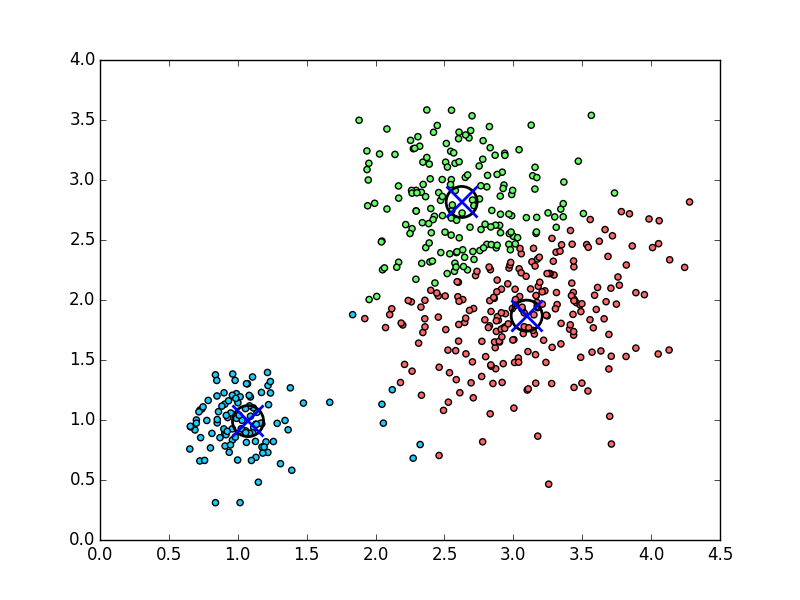
\includegraphics[width=0.80\textwidth]{pic/kmeans.png}
	\caption{An example result for K-means algorithm.}
	\label{fig:kmeans}
\end{figure}

An example result for $K-means$ algorithm is show in figure \ref{alg:kmeans}. The final clusters is divided by the centroids.
When performing the $K-means$ algorithm, one can experiment with different value of $k$, and draw a graph about the size of $k$ and the $L_2$-norm value. One can expect that, when first increase the $k$ value, the $L_2$-norm value would decrease sharply, and after some bigger $k$, the $L_2$-norm would stop or decrease with a small slope. And turning point is usually chose as a good $k$ value.

$K-means$ algorithm is simple and straightforward. However its also has some drawbacks,

\begin{itemize}
	\item The final result is heavily based on the initial centroid points
	\item May come up with local optimum value
	\item Sensitive to outliers
	\item Not suitable for big data
	\item Not apply to categorical data
\end{itemize}

The distance based method is sensitive to outliers, to overcome this, research also invented density-based partition. In density-based partition, clusters are define as a connected group and is able to make up the clusters in arbitrary shape. Due to this property, density-based partition clustering algorithm does not influence by the outliers.

%TODO or not discuss about density based algorithm in detail.

\section{Hierarchical Clustering Algorithm}

Hierarchical clustering is developed to build a cluster hierarchy, meaning, a cluster tree, people may refer it as $dendrogram$. An example of dendrogram is shown in figure \ref{fig:a_dendrogram}. Not like partition based clustering, the $dendrogram$ made by hierarchical clustering can be cut at any stage, thus enable researchers explore the data in different levels. Hierarchical clustering methods can be divided into two aspects, agglomerative and divisive. The agglomerative way, or called the bottom-up method, created the $dendrogram$ by iteratively join the most similar two object into one. And the divisive method treats the whole dataset as one object, and recursively divide the object into pieces.

\begin{figure}
	\centering
	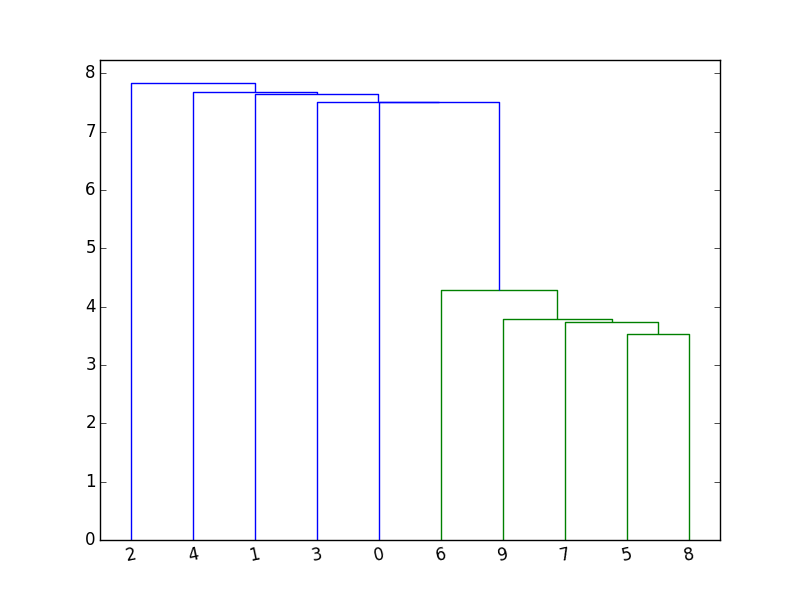
\includegraphics[width=0.80\textwidth]{pic/dendrogram.png}
	\caption{An example of a dendrogram.}
	\label{fig:a_dendrogram}
\end{figure}

The following part illustrates the essential component of Agglomerative Hierarchical Clustering(AHC). The naive AHC algorithm starts with treating every point in the dataset as individual cluster, and repeated merge the closest objects into one, until there is only on big component left. Algorithm \ref{alg:primitiveHAC} shows the primitive AHC algorithm.

\algrenewcommand\Return{\State \algorithmicreturn{} }% http://tex.stackexchange.com/questions/69449/avoid-putting-statements-on-the-same-line-with-algorithmicx
\begin{algorithm}[h]
	\caption{Primitive AHC algorithm}
	\label{alg:primitiveHAC}
	\begin{algorithmic}[1]
		\Procedure{primitive AHC}{s,D}
		
		\State $S_{origin} \leftarrow S$
		\State $n \leftarrow \lvert S \rvert$
		\State $den \leftarrow \left[\right]$
		\State $size[x] \leftarrow 1, $ for all $x \in S$
		\For{$i \leftarrow 0, \dots , n - 2 $}
		\State $(I,J) = argmin_{(SxS)\setminus \Delta} D$
		\State append (I,J) to den
		\State $S \leftarrow S \setminus \left\{I,J\right\} $
		\State Create a new label $L$, $L \notin S \cup S_{origin}$
		\State \begin{varwidth}[t]{\linewidth}
			Update the matrix containing the distances
			\par\hskip\algorithmicindent $D[L,x] = D[x,L] = \text{FORMULA} ( D[I,x], D[b,J],$ 
			\par\hskip\algorithmicindent $D[I,J], size[I], size[J]) $,  for all $x \in S$
		\end{varwidth}
		\State $size[L] \leftarrow size[I] + size[J]$
		\State $S \leftarrow S \cup \left\{L\right\}$
		\EndFor 
		
		\Return den
		\EndProcedure
		
		The $\text{FORMULA}$ is the updating formula used for the chosen linkage, while $d$ is the distance metric. Note that our notation somewhat freely uses $I$ and $J$ to mean either the label of the cluster or the cluster itself.
	\end{algorithmic}
\end{algorithm}

The formula for updating the distance is usually selected between single, complete, average, weighted, Ward, centroid and median linkage(details in \cite{mullner2012fastcluster}). Average distance is described below:

\begin{definition}[Average distance]
	\label{def:average_distance}
	Given a distance measure $D$, the average distance, $Average_D$, for cluster $A$ and $B$ is defined as
	\[
	D_A \left(A, B \right) = \frac{
			\sum\limits_{i=1}^{\lvert  A\rvert } \sum\limits_{j=1} \lvert B \lvert D \left(A_i, B_j \right)		
		}{
			\lvert A \lvert	\lvert B \lvert
		}
	\]
\end{definition}


\begin{definition}[Average Updating Formula]
	\label{def:average_updating}
	Given that cluster $A$ and $B$ join together, the distance between any other cluster $M$ to the joined cluster could be update as
	\[
	\frac{
		n_{A,M} D_A \left( A, B \right) + n_{B,M} D_A \left( B, M \right)
		}{
		n_{A, M} + n_{B,M}
		}
\]
\end{definition}


Despite the advantages that, AHC can apply to any distance measure and suit any type of attribute type, when facing big data problem, the time complexity, $O(n^3)$, makes it impossible to finish compute.


\chapter{Approximate Hierarchical Clustering Algorithm}

As discussed in the previous chapter, the time complexity of a traditional accurate hierarchical clustering algorithm is $O(n^3)$. However, the datasets size of today's application domain has dramatically increased. Conducting a traditional agglomerative hierarchical clustering on such dataset would not be proper for an expected running time.

To handle the scaling challenge, researchers found two approaches. At fist, researchers are focused on how to find faster algorithms which generate the same hierarchical tree as the original algorithm. The hardworking of the first approach came to its limit, when dataset scale becomes even lager. The later contribution turns to find a approximate hierarchical clustering algorithm, which is not consistency to but closely resembles the exact algorithms. 

This chapter will mainly discuss the current research in the approximate hierarchical clustering algorithms. 

\section{Experiment and Comparison Difficulty}

Before the discussion of the approximate algorithms, an brief illustration about the difficulty of experiment and comparison of such approximate hierarchical clustering algorithms.

%TODO this part could refer to the covernote

\section{Algorithm by Patra}

Patra et al.~\cite{patra2010distance}  proposed a method, l-AL for AHC to deal with large dadtasets problem with average linkage. In their work, a set of leaders are proposed to represent the whole datasets, which are then applied the standard average link method. The advantage is that this method works for any distance metric, and reduces the running complexity as it is not requested to store the whole  dataset in to memory, only the leaders are retained. 

To perform a $l-AL$ algorithm \cite{hartigan1975clustering}, firstly, a set of leaders should be chose, and a standard average linkage method will be implement inside each group. The average linkage method has been discussed in the previous chapter. The focus below will be mainly about the way they used to choose leaders from the origin dataset.

\algrenewcommand\Return{\State \algorithmicreturn{} }
\begin{algorithm}[h]
	\caption{Leaders Selecting algorithm}
	\label{alg:selectLeader}
	\begin{algorithmic}[1]
		\Procedure{leaderSelect}{dataset, $\tau$}
		\State leaders $\leftarrow$ empty hash map of node and set of nodes
		\For{$i \leftarrow dataset$}
			\State \text{IF}  exists a $l$ in $leaders$, and $ || l - i || < \tau $
			\State \hskip\algorithmicindent put current node $i$ into the set in $leaders$ with key $i$.
			\State \text{ELSE}
			\State \hskip\algorithmicindent make i a new leader, put an empty set into $leaders$ with key $i$
		\EndFor		
		\Return $leaders$
		\EndProcedure

	This algorithm takes two input, one is the whole dataset which is used in the hierarchical clustering, the other one is a tolerante value $\tau$. The return value is the chosen leaders with their attached nodes.
	\end{algorithmic}
\end{algorithm}

A traditional way of finding leaders is shown in Algorithm\ref{alg:selectLeader}. The size of leaders is determined by the dataset itself and also largely on the parameter $\tau$. The time complexity is $O(mn)$.

In the article by Patra et al.~\cite{patra2010distance}, the author introduced a more efficient way to compute the leaders. An algorithm called $Accelerating Leaders$ is proposed, which take the use of triangle inequality property and reduce the iteration when computing leaders. The detail of this $Accelerating Leaders$ algorithm is not mentioned here, as it is not the essential part of this paper, one can easily refer to the paper.
%TODO: no, I think you should reproduce it. 


The $l$-AL algorithm is based on the leader selection and average linkage to perform the clustering. 
Algorithm \ref*{alg:lal} shows how to perform the $l$-AL, with a time complexity $O(mn + m^2)$ = $O(mn)$ and a space complexity $O(m^2)$.
Compared to the traditional AL algorithm, $l$-AL algorithm does not perform the hierarchy clustering method on the whole dataset, which reduce the computation pressure. 
As the author discussed about, the $l$-AL may overestimate or underestimate the distance between different clusters.
However, for larger datasets, the members of each leader is also big, which will make the members will distributed.


\algrenewcommand\Return{\State \algorithmicreturn{} }
\begin{algorithm}[h]
	\caption{$l$-AL}
	\label{alg:lal}
	\begin{algorithmic}[1]
		\Procedure{$l$-AL}{$s$, $\tau$, $h$}
		\State Apply leader selection algorithm \ref{alg:selectLeader} on $s$, get a map $leadersMap$, get keys out from $leadersMap$ as $L$.
		\State Apply average linkage algorithm AL($L$, $h$), to get a hierarchical cluster $HC$.
		\State Replace each leader in $HC$ with a set of nodes in $leadersMap$
		\State Thus, $HC$ becomes a sequence of clustering dataset $result$
		\Return $result$
		\EndProcedure
		
		This algorithm takes three inputs, a raw dataset $s$, two tuning parameters, $tau$ and $h$.
	\end{algorithmic}
\end{algorithm}

%TODO You can include an illustration as well, perhaps showing how leaders might be selected or a dendrogram showing the leaders



\section{Algorithm by Gilpin}
3.2 Algorithm by Gilpin et. al

\section{Twister Tries Approach}
3.3 Twister tries + the extension I worked on later

\section{Comparison}
3.4 Some comparison (this can also be done directly in the section, but it might be easier to do it separatly)

\chapter{Conclusion}

\printbibliography

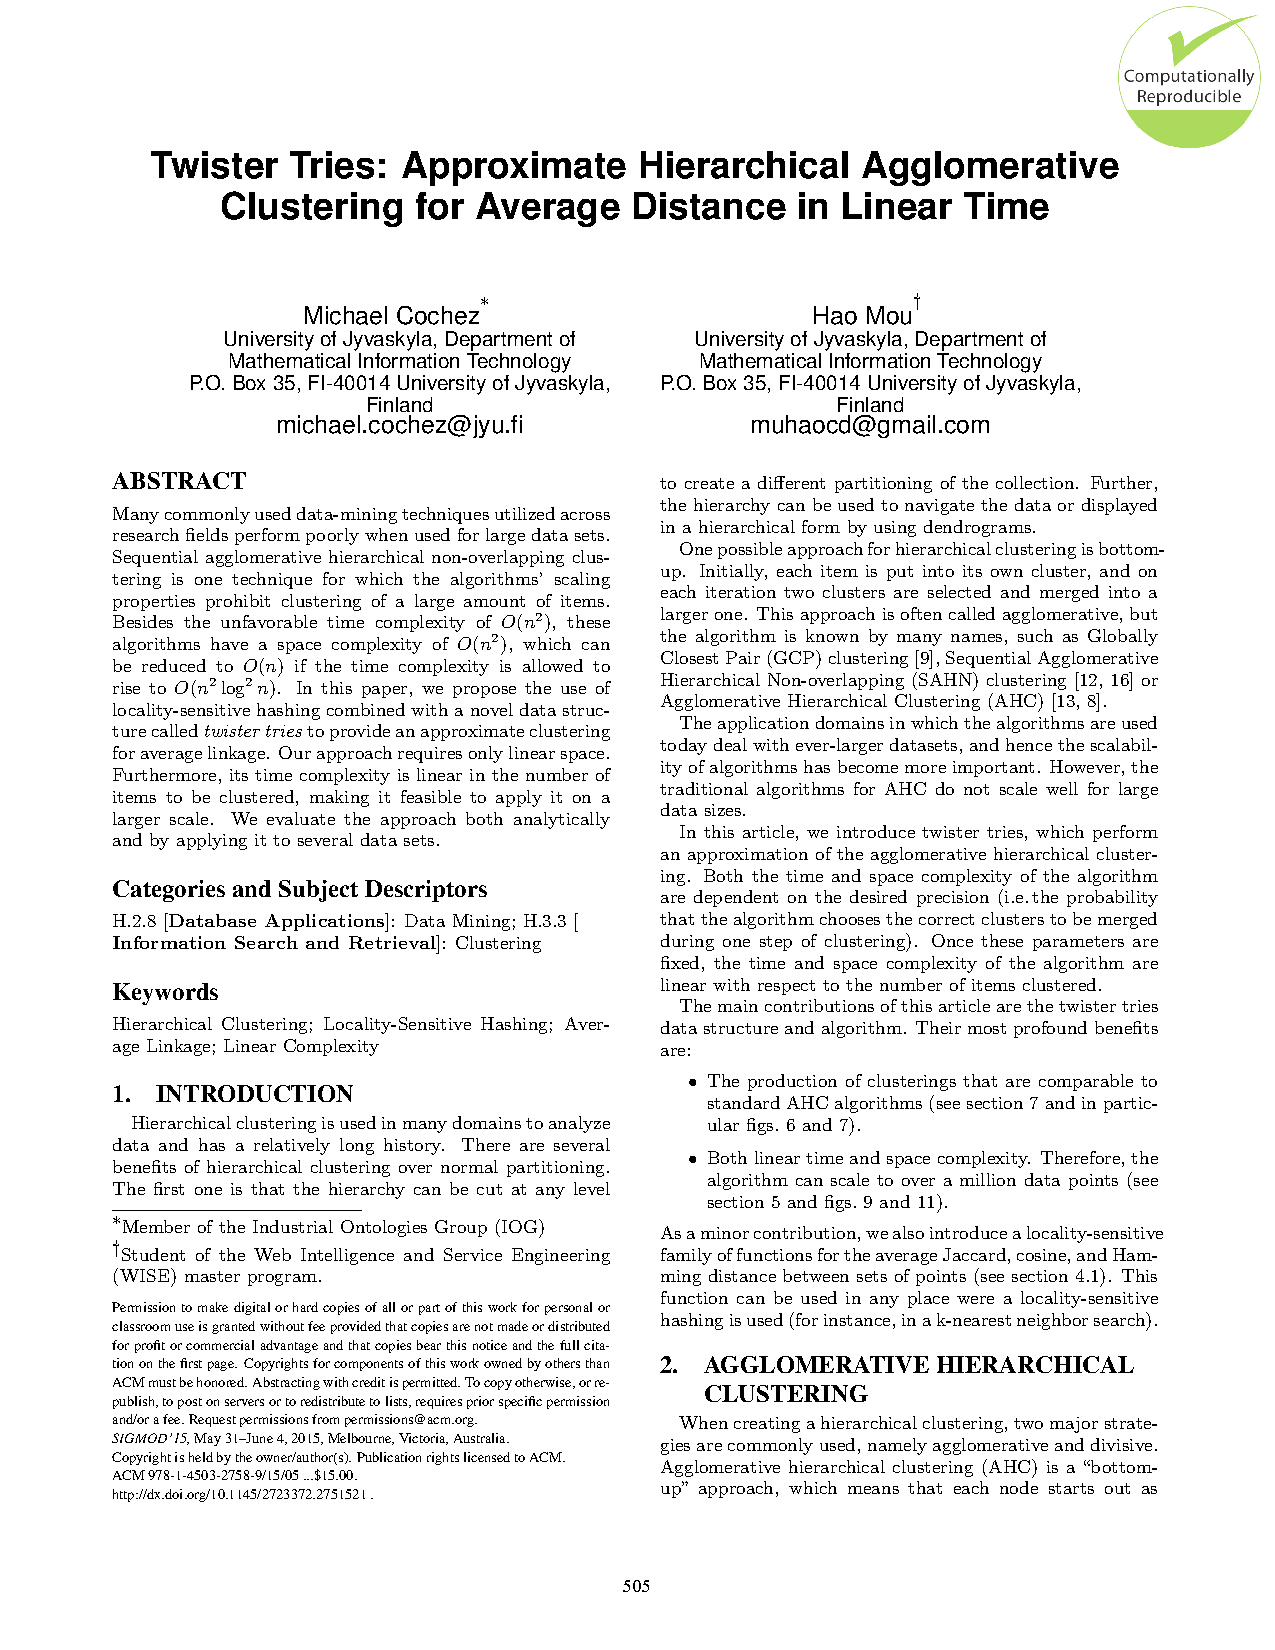
\includepdf[pages={-}]{twister_tries_reproducible.pdf}




\appendix

\section{The article}
Appendix: the article

\end{document}
